


\documentclass[11pt]{article}
\usepackage[margin=1in]{geometry}
\usepackage{fancyhdr}
\usepackage{amsmath , amsthm , amssymb}
\usepackage{graphicx}
\usepackage{hyperref}
\usepackage{authblk}
\usepackage{setspace}

\usepackage{lscape} %this is to make the landscape of individual table pages.
\usepackage{enumitem, float, booktabs}
\setcounter{MaxMatrixCols}{10}

\pagestyle{fancy}
\lhead{}
\chead{}
\rhead{}
\lfoot{}
\cfoot{\thepage}
\rfoot{}
\setlength{\parindent}{0.5in}
\geometry{left=.8in,right=1in,top=1in,bottom=1in}
\renewcommand{\baselinestretch}{2}
\usepackage[usenames,dvipsnames]{xcolor}

\definecolor{pine_green}{rgb}{0.0, 0.47, 0.44}

\begin{document}

\begin{onehalfspacing}

\begin{center}
\textbf{EC 320: Introduction to Econometrics} \bigskip

\textbf{Problem Set\bigskip\ 4}
\bigskip
\end{center}


\noindent \textbf{Total: points}

\noindent \textbf{Due: }

\bigskip

\noindent \textbf{Learning Outcomes:}
\begin{itemize}
\item Understanding hypothesis testing
\item Understanding multiple regression models
\item Understanding goodness of fit 
\end{itemize}

\bigskip


\noindent \textbf{Checklist Before Handing In:}
\begin{itemize}
\item Did you answer all questions?
\item Did you answer all parts for each question?
\item Were your answers too vague? If so, make them more precise to make sure they really answer the question being asked.
\end{itemize}

\bigskip

\noindent {\textbf{Instructions:}}\ You are encouraged to work with other students in the class, but you must provide original responses. To receive full credit, justify your answers and list your collaborators. For full credit on the computational exercises, include your code and output in addition to your answers. You will turn in digital copies of your responses on Canvas. Please note the list of acceptable file types on the submission page.  \\
\vspace{0.1in}

Name: 			\\
\vspace{0.1in}

Collaborator 1: \\

\vspace{0.1in}

Collaborator 2: \\
	
\vspace{0.1in}

Collaborator 3: 		
			

\newpage


\begin{center}
\textbf{Analytical Questions} \bigskip
\end{center}

\begin{enumerate}
	
\item Suppose that you run a regression of $Y_i$ on $X_i$ with 102 observations and obtain an estimate for the slope (\textit{i.e.,} $\hat{\beta}_2$). Your estimate for the standard error of $\hat{\beta}_2$ is 1. You are considering two different hypothesis tests. 

The first is a \textbf{one-sided test}:
$$\text{H:}_0 \enspace \beta_2 = 0, \quad \text{H:}_a \enspace \beta_2 > 0, \quad \alpha = 0.05.$$

The second is a \textbf{two-sided test}:
$$\text{H:}_0 \enspace \beta_2 = 0, \quad \text{H:}_a \enspace \beta_2 \neq 0, \quad \alpha = 0.05.$$

\begin{enumerate}
	\item What values of $\hat{\beta}_2$ would lead you to reject the null hypothesis in the \textbf{one-sided} test?\\
	
		{\color{pine_green} You reject $\text{H}_0$ if $t > t_\text{crit}$. 
		
		Given $102 - 2$ degrees of freedom, you will find on your table that $t_\text{crit} = 1.66$.
		
		The $t$-statistic is $t = \dfrac{\hat{\beta}_2}{\mathop{\text{SE}}(\hat{\beta}_2)} = \dfrac{\hat{\beta}_2}{1}$.
		
		You will reject $\text{H}_0$ if $\hat{\beta}_2 > 1.66$.\\
		
	}
	
	\item What values of $\hat{\beta}_2$ would lead you to reject the null hypothesis in the \textbf{two-sided} test?\\
	
		
	{\color{pine_green} You reject $\text{H}_0$ if $|t| > t_\text{crit}$. 
		
		Given $102 - 2$ degrees of freedom, you will find on your table that $t_\text{crit} = 1.984$.
		
		The $t$-statistic is $t = \dfrac{\hat{\beta}_2}{\mathop{\text{SE}}(\hat{\beta}_2)} = \dfrac{\hat{\beta}_2}{1}$.
		
		You will reject $\text{H}_0$ if $\hat{\beta}_2 > 1.984$ or $\hat{\beta}_2 < -1.984$.\\
		
	}
	\item What values of $\hat{\beta}_2$ would lead you to reject the null hypothesis in the \textbf{one-sided} test, \textbf{but not} the \textbf{two-sided} test?\\
	
	{\color{pine_green} You will reject $\text{H}_0$ in a one-sided test if $\hat{\beta}_2 > 1.66$. 
		
		You will fail to reject $\text{H}_0$ in a two-sided test if $-1.984 \leq \hat{\beta}_2 \leq 1.984$. 
		
		If $1.66 \leq \hat{\beta}_2 \leq 1.984$, then you will reject $\text{H}_0$ in the one-sided test, but not in the two-sided test.\\
	}

	\item What values of $\hat{\beta}_2$ would lead you to reject the null hypothesis in the \textbf{two-sided} test, \textbf{but not} the \textbf{one-sided} test?\\
	
		{\color{pine_green} You will fail to reject $\text{H}_0$ in a one-sided test if $\hat{\beta}_2 \leq 1.66$. 
		
		You will reject $\text{H}_0$ in a two-sided test if $\hat{\beta}_2 > 1.984$ or $\hat{\beta}_2 < -1.984$. 
		
		If $\hat{\beta}_2 < -1.984$, then you will reject $\text{H}_0$ in the two-sided test, but not in the one-sided test.\\
	}
\end{enumerate}


\item Suppose that you are studying the effect of police officers on crime rates in several large American cities. When you estimate the model
$$\text{Crime}_i = \beta_1 + \beta_1 \text{Police}_i + u_i,$$
you obtain a positive slope estimate.

\begin{enumerate}
	\item What does your slope estimate imply about how the number of police officers affects crime?\\
	
	
	{\color{pine_green}
		The positive slope estimate ($\hat{\beta}_1$) suggests that crime increases as the number of police increase. In other words, ``more police, more crime.''\\
	}
	
	\item Provide an example of an omitted variable that could explain why the slope estimate is positive. \\
	
	{\color{pine_green}
		The idea here is to think of a variable that---if omitted from a regression of crime on police---would bias the slope estimator upwards. There are many examples that you could give, but they need to produce positive omitted-variable bias. If the variable is called $\text{Omitted}_i$, then the bias from omitting $\text{Omitted}_i$ is given by
		$$\text{Bias} = \beta_{\text{Omitted}} \frac{\mathop{\text{Cov}}(\text{Police}_i, \text{Omitted}_i)}{\mathop{\text{Var}}(\text{Police}_i)}.$$
		
		For $\text{Bias}>0$, there are two types of omitted variables that you could describe: either 1) the omitted variable is positively correlated with crime (\textit{i.e.}, $\beta_{\text{Omitted}} > 0$) and positively correlated with police or 2) it is negatively correlated with crime (\textit{i.e.}, $\beta_{\text{Omitted}} < 0$) and negatively correlated with police. (If it is negatively correlated with one variable, but positively correlated with the other, then $\text{Bias}<0$.)
		
		One example of an omitted variable that could cause positive bias is the number of ex-convicts. For a variety of reasons, those who have been convicted of a crime are more likely to commit a new crime than those who have never been convicted, so cities with more ex-convicts are likely to exhibit higher crime rates. One might also expect officials in cities with more ex-convicts to recognize that fact and respond by hiring more police.\\
	}
	
\end{enumerate}


\item Suppose that your friend wrote a computer program that runs both simple and multiple linear regressions using OLS. Your friend asks you to test the software. After importing a dataset with 2000 observations and three cryptically named variables---$Y$, $X_1$, and $X_2$---you run two regressions. The first is a regression of $Y$ on $X_1$, which gives you an intercept estimate of 10.4, a slope estimate of -3.8, and $R^2 = 0.215$. The second is a regression of $Y$ on $X_1$ and $X_2$, which gives you an intercept estimate of 9.3, an $X_1$ slope estimate of -2.9, an $X_2$ slope estimate of -0.07, and $R^2 = 0.198$. You tell your friend that they must made a mistake somewhere in their code. Why?\\


{\color{pine_green}
	The model with fewer variables had a higher $R^2$, which contradicts what we learned in class. If the model contains only one variable, then $R^2$ tells us the percentage of the variation in $Y$ explained by $X$. If the model contains more than one variable, then $R^2$ tells us the percentage of the variation in $Y$ explained by all of the variables in the model, collectively. All else being equal (\textit{e.g.,} the dependent variable, sample size, \textit{etc.}), adding explanatory variables to a regression generally increases $R^2$. In the edge case where an additional variable explains none of the variation in $Y$, then $R^2$ will not change. However, there is no case in which $R^2$ will decrease. You can illustrate this idea using Venn diagrams.
	
	The orange circle describes the variation in $Y$, and the red circle describes the variation in $X_1$. In the simple linear regression, the overlap between the orange and red circles describes the variation in $X_1$ that explains $Y$.
	
	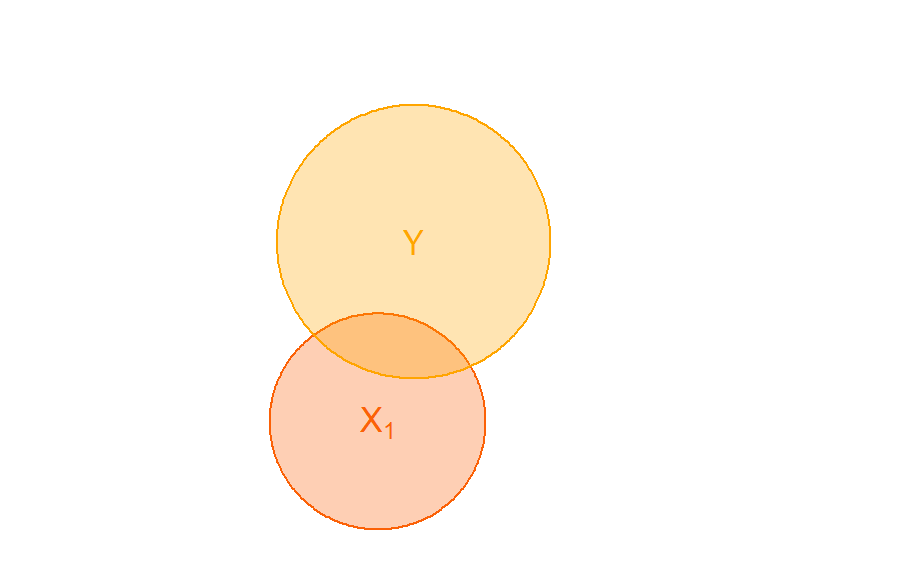
\includegraphics[width=0.85\textwidth]{R2_base.png}
	
	Adding $X_2$ to the regression provides an additional region of overlap: the overlap between the orange and gray circles describes the variation in $X_2$ that explains $Y$. The important thing to notice is that---compared to the simple linear regression---more of the variation in $Y$ is explained by the $X$ variables. In other words, $R^2$ has increased.
	
	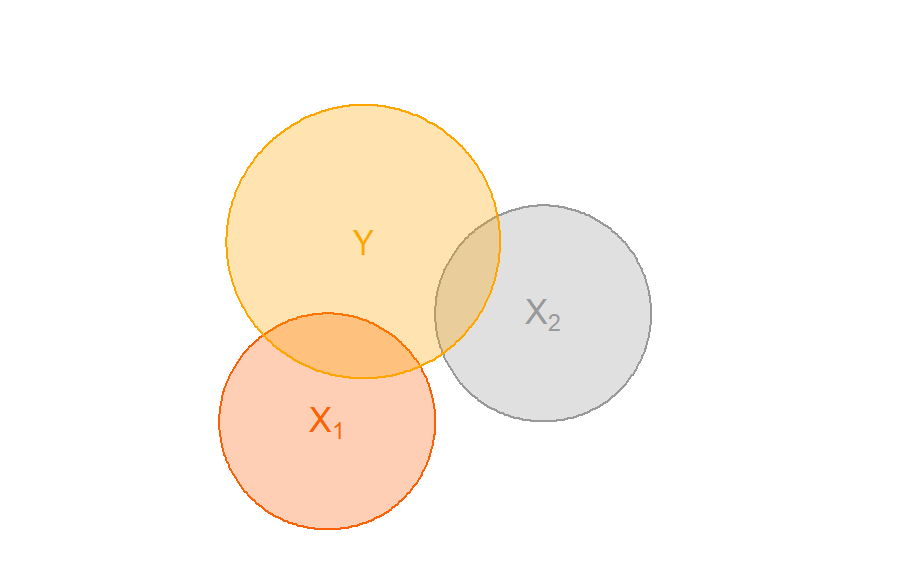
\includegraphics[width=0.85\textwidth]{R2_case1.png}
	
	However, if $X_2$ is irrelevant in the sense that it explains none of the variation in $Y$, then the multiple regression model will not explain any more of the variation in $Y$ than the simple regression model. In this case $R^2$ does not change by adding $X_2$.
	
	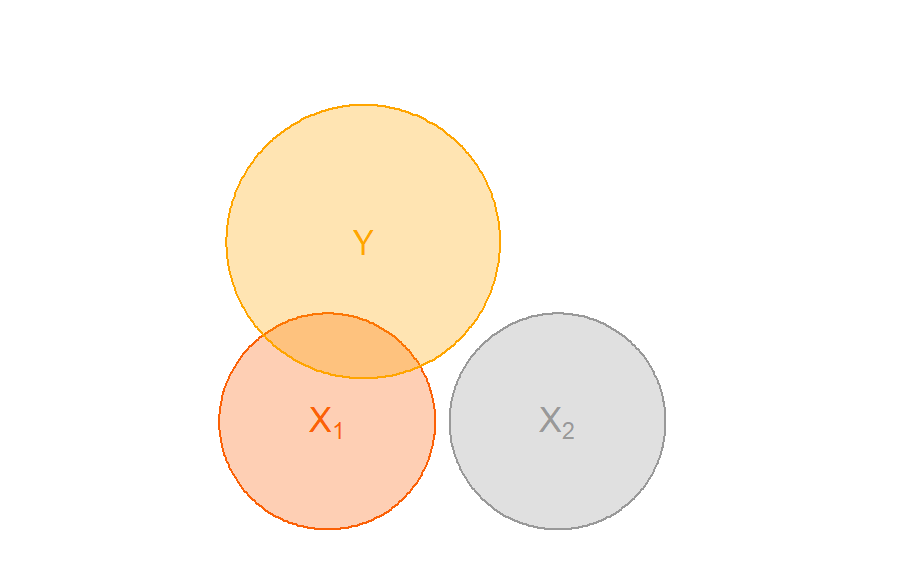
\includegraphics[width=0.85\textwidth]{R2_case2.png}
	
	There is no way for me to add a variable that ``un-explains'' $Y$. I can't erase any of the existing overlap between $X_1$ and $Y$ by adding $X_2$. In other words, $R^2$ cannot decrease.\\
}

\item A useful application of multiple regression analysis is \textit{Hedonic modeling}. Hedonic models seek to explain the price of a good---such as a house---in terms of its attributes (\textit{e.g.,} number of bedrooms, square footage, or distance from the nearest toxic waste dump). Consider the following Hedonic model of home sale prices:
$$\text{Price}_i = \beta_0 + \beta_1 (\text{Square footage})_i + \beta_2 \text{Bathrooms}_i  + \beta_3 \text{Bedrooms}_i + u_i.$$
Using data from 37 home sales, you estimate the model and obtain $\hat{\beta}_0 = 90000$, $\hat{\beta}_1 = 1100$, $\hat{\beta}_2 = 16000$, $\hat{\beta}_3 = 35000$, $\mathop{\text{SE}}(\hat{\beta}_1) = 650$.

\begin{enumerate}
	\item Interpret each coefficient.\\
	
		{\color{pine_green} $\hat{\beta}_0$: The average sale price of an empty lot (\textit{i.e.}, a home with zero square footage, zero bedrooms, and zero bathrooms) is \$90,000.
		
		$\hat{\beta}_1$: Holding the number of bedrooms and the number of bathrooms constant, each additional square foot of living space increases a home's sale price by \$1,100, on average.
		
		$\hat{\beta}_2$: Holding the number of bedrooms and square footage constant, each additional bathroom increases a home's sale price by \$16,000, on average.
		
		$\hat{\beta}_3$: Holding the number of bathrooms and square footage constant, each additional bedroom increases a home's sale price by \$35,000, on average.\\
	}
	
	\item What is the model's forecasted sale price for a 2500-square-foot home with 3 bedrooms and 2.5 bathrooms?\\
	
		{\color{pine_green} The forecasted price is \$2,985,000:
		\begin{align*}
		\hat{\text{Price}}_i &= 90000 + 1100 \cdot (2500) + 16000 \cdot (2.5) + 35000 \cdot (3) \\
		&= 2985000.\\
		\end{align*}
	}
	
	\item In a remodeling frenzy, a homeowner adds an additional bedroom and an additional bathroom by splitting up existing rooms. What is the forecasted change in the price of her home?\\
	
		{\color{pine_green} The forecasted change in price is \$51,000:
		\begin{align*}
		\Delta\hat{\text{Price}}_i &= \hat{\beta}_2 \cdot \Delta\text{Bathrooms}_i + \hat{\beta}_3 \cdot \Delta\text{Bedrooms}_i \\
		&= 16000 \cdot (1) + 35000 \cdot (1) \\
		&= 51000.
		\end{align*}
		Alternatively, you could have started with the house described in part (b) and added 1 bedroom and 1 bathroom. Then you could have taken the difference in forecasted prices between the remodeled home and the original home to obtain the expected change in sale price. This alternative approach yields the same forecasted change in price demonstrated above.\\
	}
	
	\item A homeowner adds a 450-square-foot bedroom and a 75-square-foot bathroom by extending the footprint of his home into an area that used to be a driveway. What is the forecasted change in the price of his home? \\
	
		{\color{pine_green} The forecasted change in price is \$628,500:
		\begin{align*}
		\Delta\hat{\text{Price}}_i &= \hat{\beta}_1 \cdot \Delta (\text{Square footage})_i + \hat{\beta}_2 \cdot \Delta\text{Bathrooms}_i + \hat{\beta}_3 \cdot \Delta\text{Bedrooms}_i \\
		&= 1100 \cdot(525) + 16000 \cdot (1) + 35000 \cdot (1) \\
		&= 628500.
		\end{align*}
		Alternatively, you could have started with the house described in part (b) and added 525 square feet, 1 bedroom, and 1 bathroom. Then you could have taken the difference in forecasted prices between the remodeled home and the original home to obtain the expected change in sale price. This alternative approach yields the same forecasted change in price demonstrated above.\\
	}
	
	\item Conduct two-sided tests of the hypothesis that square footage has no effect on sale price at the 10, 5, and 1 percent levels.\\
	
	{\color{pine_green} Here, I'm telling you to test the null hypothesis 
		$$\text{H}_0: \beta_1 = 0$$ 
		against the alternative hypothesis 
		$$\text{H}_a: \beta_1 \neq 0$$ 
		at $\alpha = 0.1$, $\alpha = 0.05$, and $\alpha = 0.01$.
		
		For each of these tests, you will use the same $t$ statistic:
		\begin{align*}
		t &= \dfrac{\hat{\beta}_1 - \beta_1^0}{\mathop{\text{SE}}(\hat{\beta}_1)} \\
		&= \dfrac{\hat{\beta}_1 - 0}{\mathop{\text{SE}}(\hat{\beta}_1)} \\
		&= \dfrac{1100}{650} \\
		&\approx 1.69.
		\end{align*}
		
		You also need to find three different critical values of $t$ (\textit{i.e.}, $t_{\text{crit}}$). Each of these will have the same degrees of freedom:
		
		$$\text{dof} = n - k - 1 = 37 - 3 - 1 = 33.$$
		
		Your table does not have a row for 33 degrees of freedom, so ``play it safe'' by picking $t_{\text{crit}}$ with 30 degrees of freedom. Doing this ensures that the Type I error rate of your tests does not exceed the chosen significance levels (the $\alpha$s).
		
		For  $\alpha = 0.1$, $t_{\text{crit}} = 1.697$.
		
		For  $\alpha = 0.05$, $t_{\text{crit}} = 2.042$.
		
		For  $\alpha = 0.01$, $t_{\text{crit}} = 2.75$.
		
		You will reject the null hypothesis if $|t| > t_{\text{crit}}$.
		
		For the 10 percent test, $|t| = 1.69 > t_{\text{crit}} = 1.697$ is false. This implies that you fail to reject the null hypothesis at the 10 percent level.
		
		The other two $t_{\text{crit}}$s are greater than 1.697, which implies that you will also fail to reject the null hypothesis at the 5 percent and 1 percent levels.\\
	}

	\item  Construct a 95 percent confidence interval for $\beta_1$.\\
	
		{\color{pine_green}
		The 95 percent confidence interval for $\beta_1$ is outlined by 
		
		$$\hat{\beta}_1 \pm t_{\text{crit}} \cdot \mathop{\text{SE}}(\hat{\beta}_1).$$
		
		The appropriate $t_{\text{crit}}$ is 2.042 (based on 30 degrees of freedom and $\alpha = 0.05$ for a two-sided test).
		
		Then the confidence interval for $\beta_1$ is outlined by
		
		$$1100 \pm 2.042 \cdot 650.$$
		
		Then the 95 percent confidence interval for $\beta_1$ is 
		
		$$-227 < \beta_1 < 2,427.$$
		

	}

\end{enumerate}

\end{enumerate}

\clearpage

\section*{Computational Problems}

For this portion of the problem set, you will use the \texttt{apple.csv} file in the \texttt{Problem Set 4} folder on Canvas. The file contains data from an experimental survey. The survey presented participants with \textbf{randomly determined} prices for ``eco-labeled'' apples and regular apples and then asked how many eco-labeled and regular apples they would buy at those prices. For reference, eco-labeling helps consumers identify sustainably-produced (or ``green'') products and helps firms command higher prices for their products. You will estimate the demand for eco-labeled and regular apples by running regressions of apple quantity on prices. The fact that the prices were randomly assigned means that the exogeneity assumption holds---so long as both prices are included in the model. To complete this assignment, you will need to load the \texttt{tidyverse}, \texttt{stargazer}, and \texttt{broom}. Use \texttt{Problem\_Set\_04\_template.Rmd} as a template.

\begin{table}[htb]
	\centering
	\begin{tabular}{@{\extracolsep{1cm}} l l @{}}
		\toprule
		\textbf{Variable Name} & \textbf{Description}  \\ \toprule
		\texttt{reglbs} & Pounds of regular apples demanded \\
		\texttt{ecolbs} & Pounds of eco-labeled apples demanded \\
		\texttt{regprc} & Price of regular apples (per pound) \\
		\texttt{ecoprc} & Price of eco-labeled price (per pound) \\
		\bottomrule
	\end{tabular}
\end{table}

\begin{enumerate}
	
\item Run a regression of \texttt{reglbs} on \texttt{regprc}. Interpret the slope coefficient. Is the sign of the slope consistent with what you know about demand curves?
\item Run a regression of \texttt{ecolbs} on \texttt{ecoprc}. Interpret the intercept coefficient.
\item Run a regression of \texttt{reglbs} on \texttt{regprc} and \texttt{ecoprc}. How does the estimated coefficient on \texttt{regprc} change? What does this tell you about the correlation between \texttt{regprc} and \texttt{ecoprc}? Justify your answer and then use \texttt{R} to verify.
\item Run a regression of \texttt{ecolbs} on \texttt{regprc} and \texttt{ecoprc}. Identify and interpret $R^2$.
\item Summarize your regression results in a table. Which two of the four regressions have the highest $R^2$? Why?
\item Construct a 99 percent confidence interval for the \texttt{ecoprc} coefficient from the regression described in exercise 4.

\end{enumerate}
\end{onehalfspacing}
\end{document}
